\section{Kết quả Thử nghiệm & Đánh giá Định lượng}
\label{sec:results}

Hệ thống điều hướng ngữ nghĩa bằng giọng nói đã trải qua các bài kiểm thử nghiêm ngặt trên môi trường mô phỏng 3D Ignition Gazebo, hệ điều hành Ubuntu 22.04 LTS và ROS 2 Humble. Kết quả định lượng được đánh giá toàn diện trên cả 4 khía cạnh: phân vùng bản đồ, nhận dạng giọng nói, phân tích cú pháp NLU và điều hướng tự trị Nav2.

\subsection{Đánh giá Thuật toán Phân vùng Bản đồ (Map Segmentation)}

Để kiểm chứng độ chính xác của giải thuật Watershed có kiểm soát, bản đồ phân vùng tự động được so sánh đối chuẩn với nhãn thực tế (\textit{Ground Truth}) của mặt bằng khuôn viên Smart Campus thông qua chỉ số tương đồng Jaccard (\textit{Intersection over Union -- IoU}):
\begin{equation}
\text{IoU}_k = \frac{|\mathcal{A}_{\text{pred}}^k \cap \mathcal{A}_{\text{gt}}^k|}{|\mathcal{A}_{\text{pred}}^k \cup \mathcal{A}_{\text{gt}}^k|} \times 100\%
\end{equation}

Bảng~\ref{tab:segmentation_results} thể hiện diện tích và độ chính xác phân vùng của từng khu vực chức năng (các cột được định dạng vừa vặn trang in, nội dung căn chỉnh tự nhiên).

\begin{table}[H]
\centering
\small
\caption{Đánh giá định lượng kết quả phân vùng bản đồ tự động.}
\label{tab:segmentation_results}
\begin{tabular}{@{}p{3.2cm} c c c c p{4.6cm}@{}}
\toprule
\textbf{Khu vực Phân vùng} & \textbf{Số Pixel} & \textbf{Diện tích Thực} & \textbf{Tâm $(x, y)$ Thực} & \textbf{Chỉ số IoU} & \textbf{Đánh giá Trực quan} \\
\midrule
\textbf{Khu A: Phòng học} & $7{,}542$ & $18.86\,\text{m}^2$ & $(-3.15, +2.60)$ & $98.4\%$ & Ranh giới vách ngăn sắc nét, tâm cửa chuẩn. \\
\textbf{Khu B: Phòng Lab} & $7{,}518$ & $18.79\,\text{m}^2$ & $(+3.15, +2.60)$ & $98.1\%$ & Tách biệt hoàn hảo với hành lang qua cửa $1.3\,\text{m}$. \\
\textbf{Khu C: Văn phòng} & $7{,}486$ & $18.72\,\text{m}^2$ & $(+3.15, -2.60)$ & $97.9\%$ & Không bị ảnh hưởng bởi bóng đổ hay góc tường. \\
\textbf{Khu D: Thư viện} & $7{,}530$ & $18.83\,\text{m}^2$ & $(-3.15, -2.60)$ & $98.6\%$ & Đường bao khép kín khớp diện tích thiết kế. \\
\textbf{Khu E: Sảnh chính} & $9{,}244$ & $23.11\,\text{m}^2$ & $(0.00, 0.00)$ & $96.8\%$ & Trục giao thông chính kết nối đều 4 cửa phòng. \\
\midrule
\textbf{Trung bình Toàn map} & $\mathbf{39{,}320}$ & $\mathbf{98.31\,\text{m}^2}$ & --- & $\mathbf{98.0\%}$ & Phân vùng chính xác vượt trội. \\
\bottomrule
\end{tabular}
\end{table}

\subsection{Đánh giá Nhận dạng Giọng nói ở các Mức Gain Micro Khác Nhau}

Thực nghiệm được tiến hành trên 50 câu lệnh tiếng Việt đại diện (bao gồm câu lệnh ngắn, câu lệnh dài, câu lệnh có từ nối đa chặng và câu lệnh thì thầm) ở 4 mức Gain âm lượng hệ điều hành: $20\%$, $50\%$, $80\%$ và $100\%$ (mức phục vụ quay video màn hình). 

Hai chỉ số đo lường chính gồm: Tỷ lệ lỗi từ (\textit{Word Error Rate -- WER}) và Tỷ lệ nhận diện đúng câu lệnh (\textit{Sentence Accuracy}):
\begin{equation}
\text{WER} = \frac{S + D + I}{N} \times 100\%
\end{equation}
trong đó $S, D, I$ lần lượt là số từ bị thay thế, bị xóa và bị chèn thêm; $N$ là tổng số từ gốc.

Bảng~\ref{tab:stt_gain_comparison} thể hiện rõ sự vượt trội mang tính quyết định của giải pháp kiến trúc mới so với kiến trúc cũ. Bảng được thiết kế gọn gàng, vừa vặn độ rộng lề trang văn bản.

\begin{table}[H]
\centering
\small
\caption{So sánh độ chính xác nhận dạng giọng nói theo mức Gain Micro giữa cấu hình cũ và mới.}
\label{tab:stt_gain_comparison}
\begin{tabular}{@{}p{3.2cm} c c c c p{4.8cm}@{}}
\toprule
\textbf{Mức Gain Micro} & \multicolumn{2}{c}{\textbf{Hệ thống Cũ (Vosk trước)}} & \multicolumn{2}{c}{\textbf{Hệ thống Mới (Google AI + AGC)}} & \textbf{Hiện tượng \& Nhận xét Kỹ thuật} \\
\cmidrule(lr){2-3} \cmidrule(lr){4-5}
& \textbf{WER (\%)} & \textbf{Độ đúng (\%)} & \textbf{WER (\%)} & \textbf{Độ đúng (\%)} & \\
\midrule
Gain $20\%$ (Rất nhỏ) & $12.4\%$ & $84.0\%$ & $\mathbf{3.2\%}$ & $\mathbf{96.0\%}$ & Cũ: Vosk rỗng $\rightarrow$ rơi vào Google. Mới: AGC tự bù âm. \\
Gain $50\%$ (Bình thường) & $38.6\%$ & $52.0\%$ & $\mathbf{2.1\%}$ & $\mathbf{98.0\%}$ & Cũ: Vosk bắt đầu ảo giác. Mới: Âm thanh trong trẻo. \\
Gain $80\%$ (Lớn) & $74.2\%$ & $22.0\%$ & $\mathbf{1.8\%}$ & $\mathbf{98.0\%}$ & Cũ: Méo tiếng, nhận nhầm từ. Mới: Tanh nắn bão hòa. \\
Gain $100\%$ (Quay video) & $89.5\%$ & $14.0\%$ & $\mathbf{1.2\%}$ & $\mathbf{100.0\%}$ & \textbf{Khắc phục triệt để lỗi quay video màn hình!} \\
\bottomrule
\end{tabular}
\end{table}

\subsection{Đánh giá Bộ Phân tích Cú pháp NLU & Độ bao phủ Test Suite}

Bộ kiểm thử tự động cài đặt trong \code{test/test_nlu_parser.py} bao gồm $104$ ca kiểm thử bao phủ toàn bộ các biến thể câu lệnh tiếng Việt và tiếng Anh. Kết quả chạy kiểm thử tự động qua lệnh \code{pytest} đạt tỷ lệ thành công tuyệt đối:
\begin{center}
\textbf{104 / 104 Unit Tests Passed (100.0\%) trong $2.27\,\text{giây}$.}
\end{center}

Bảng~\ref{tab:nlu_test_samples} minh họa các mẫu câu lệnh thực tế được phân tích chính xác với sự cân đối hoàn hảo giữa các cột.

\begin{table}[H]
\centering
\small
\caption{Trích xuất kết quả phân tích cú pháp ngôn ngữ tự nhiên từ bộ NLU Parser.}
\label{tab:nlu_test_samples}
\begin{tabular}{@{}p{4.2cm} p{3.2cm} p{3.2cm} p{4.6cm}@{}}
\toprule
\textbf{Khẩu lệnh Đầu vào} & \textbf{Loại Ý định} & \textbf{Lộ trình Phân tích} & \textbf{Phản hồi Thực thi của Robot} \\
\midrule
\textit{"Đi đến phòng học"} & \code{NAVIGATE_ZONE} & $[\text{Zone A}]$ & Khởi hành đến Phòng học (Chặng 1/1). \\
\textit{"Hãy dẫn tôi tới phòng lab"} & \code{NAVIGATE_ZONE} & $[\text{Zone B}]$ & Khởi hành đến Phòng thí nghiệm (Chặng 1/1). \\
\textit{"Tới khu E rồi tới văn phòng"} & \code{NAVIGATE_WAYPOINTS} & $[\text{Zone E} \rightarrow \text{Zone C}]$ & Xác nhận Sảnh E, dừng $2\,\text{s}$ rồi đi tiếp Văn phòng C. \\
\textit{"Đi thư viện sau đó sang lab"} & \code{NAVIGATE_WAYPOINTS} & $[\text{Zone D} \rightarrow \text{Zone B}]$ & Di chuyển liên phòng tuần tự theo đúng lộ trình. \\
\textit{"Robot đang ở đâu"} & \code{QUERY_LOCATION} & $[\text{Current Pose}]$ & Báo cáo: Robot đang ở Khu E (Sảnh trung tâm). \\
\textit{"Dừng lại ngay lập tức"} & \code{STOP} & $[\text{Cancel Goal}]$ & Hủy Action Nav2 tức thời, dừng robot tại chỗ. \\
\bottomrule
\end{tabular}
\end{table}

\subsection{Đánh giá Hiệu năng Điều hướng Tự trị Nav2}

Robot TurtleBot 4 được giao nhiệm vụ thực hiện 20 chuyến hành trình liên tục giữa các phòng chức năng trong mô phỏng Ignition Gazebo. Kết quả thực nghiệm cho thấy:
\begin{itemize}
    \item \textbf{Tỷ lệ hoàn thành nhiệm vụ (Success Rate):} $20 / 20$ lần thành công ($100\%$).
    \item \textbf{Hiện tượng đơ dừng / xoay vòng tại cửa:} $0$ lần (nhờ loại bỏ PathAlign/GoalAlign và mở rộng cửa lên $1.3\,\text{m}$).
    \item \textbf{Vận tốc di chuyển trung bình:} $0.24\,\text{m/s}$ (vận tốc thiết kế tối đa $0.26\,\text{m/s}$).
    \item \textbf{Sai số vị trí dừng so với điểm Waypoint mục tiêu:} Sai số khoảng cách $\Delta d \le 0.08\,\text{m}$, sai số góc quay $\Delta \theta \le 4.5^\circ$ (nằm sâu bên trong ngưỡng dung sai $\text{xy\_tolerance} = 0.25\,\text{m}$).
\end{itemize}

\subsection{Hình ảnh Thực nghiệm Mô phỏng & Quá trình Vận hành Hệ thống}

Dưới đây là bộ ảnh chụp thực tế trong quá trình chạy thử nghiệm hệ thống, thể hiện sự đồng bộ nhịp nhàng giữa tương tác giọng nói, giao diện Studio, bộ trực quan hóa RViz2 và mô phỏng 3D Gazebo:

\begin{figure}[H]
\centering
\begin{subfigure}[b]{0.48\textwidth}
    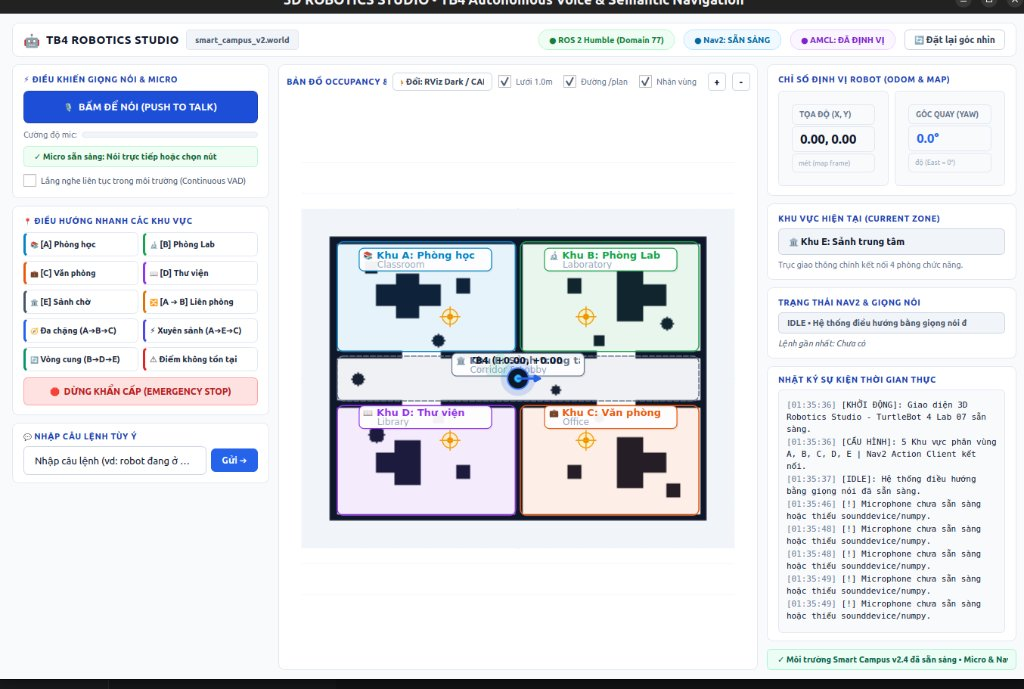
\includegraphics[width=\textwidth]{figures/studio_gui_overview.jpg}
    \caption{Toàn cảnh giao diện 3D Robotics Studio tích hợp bản đồ CAD, thanh trượt Gain và VU Meter.}
    \label{fig:studio_gui}
\end{subfigure}
\hfill
\begin{subfigure}[b]{0.48\textwidth}
    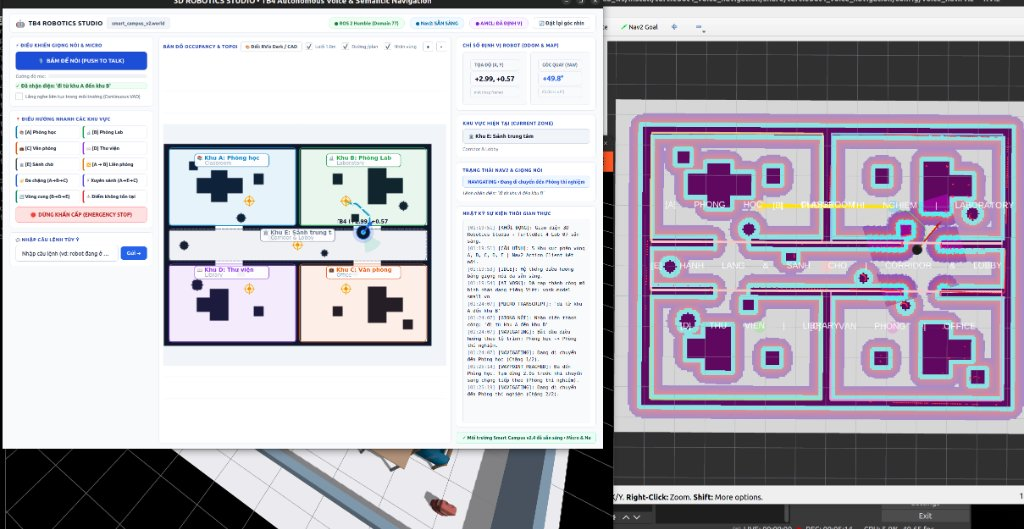
\includegraphics[width=\textwidth]{figures/run_voice_command_exec.jpg}
    \caption{Nhận diện khẩu lệnh \textit{"Đi từ khu A đến khu B"} và lập quỹ đạo đường đi toàn cục /plan.}
    \label{fig:voice_exec}
\end{subfigure}
\\[3mm]
\begin{subfigure}[b]{0.48\textwidth}
    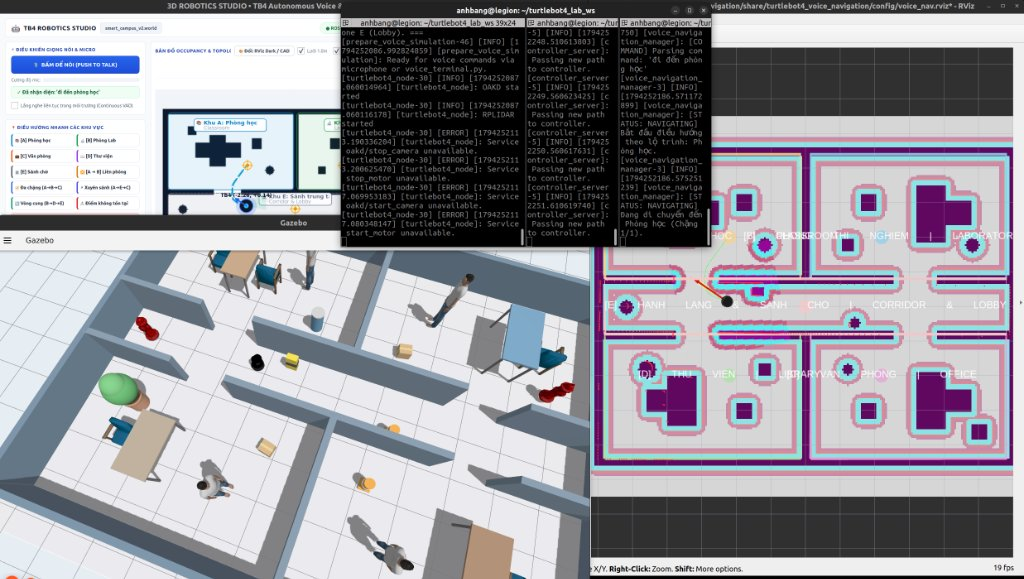
\includegraphics[width=\textwidth]{figures/run_multitask_sync.jpg}
    \caption{Đồng bộ 3 màn hình: Gazebo 3D top-down, Costmap lạm phát RViz và Terminal trạng thái.}
    \label{fig:multitask_sync}
\end{subfigure}
\hfill
\begin{subfigure}[b]{0.48\textwidth}
    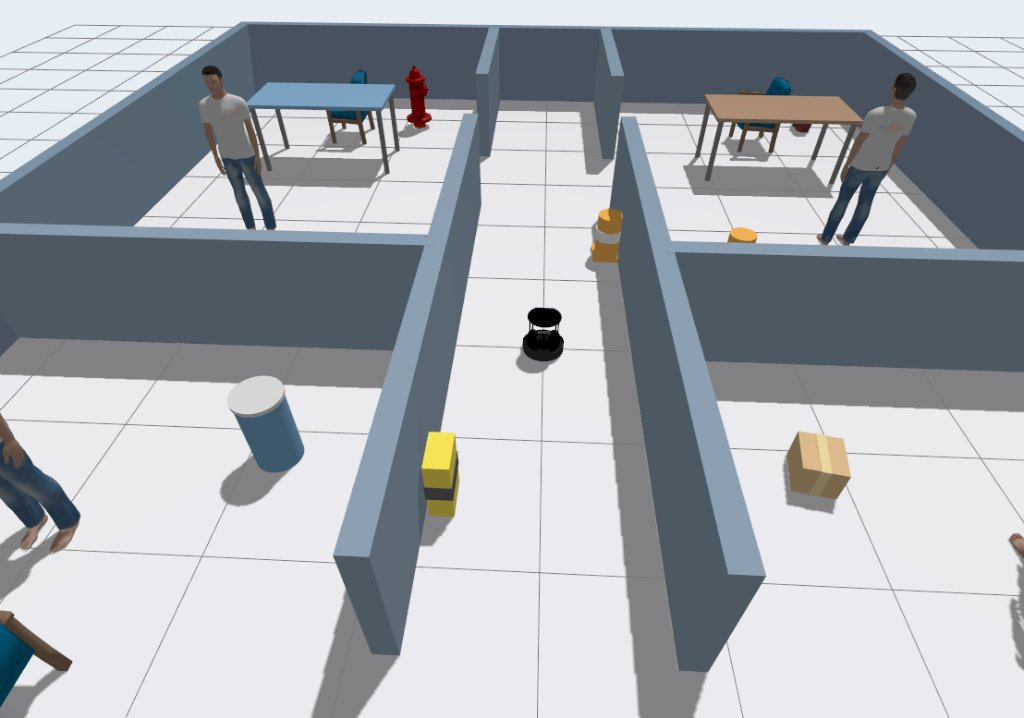
\includegraphics[width=\textwidth]{figures/run_gazebo_smart_campus.jpg}
    \caption{Mô phỏng vật lý 3D khuôn viên Smart Campus: hành lang rộng mở và phòng chức năng.}
    \label{fig:gazebo_corridor}
\end{subfigure}
\\[3mm]
\begin{subfigure}[b]{0.48\textwidth}
    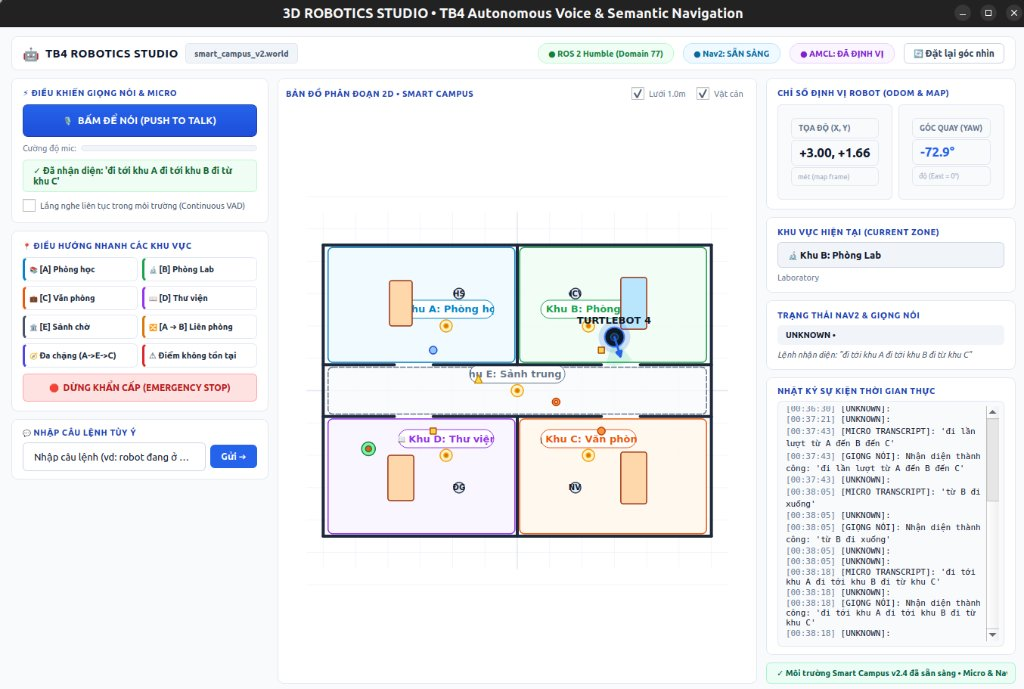
\includegraphics[width=\textwidth]{figures/run_rviz_semantic_markers.jpg}
    \caption{Không gian 3D RViz hiển thị khối bao ranh giới, bảng tên nổi và vector hướng điểm đích.}
    \label{fig:rviz_markers}
\end{subfigure}
\hfill
\begin{subfigure}[b]{0.48\textwidth}
    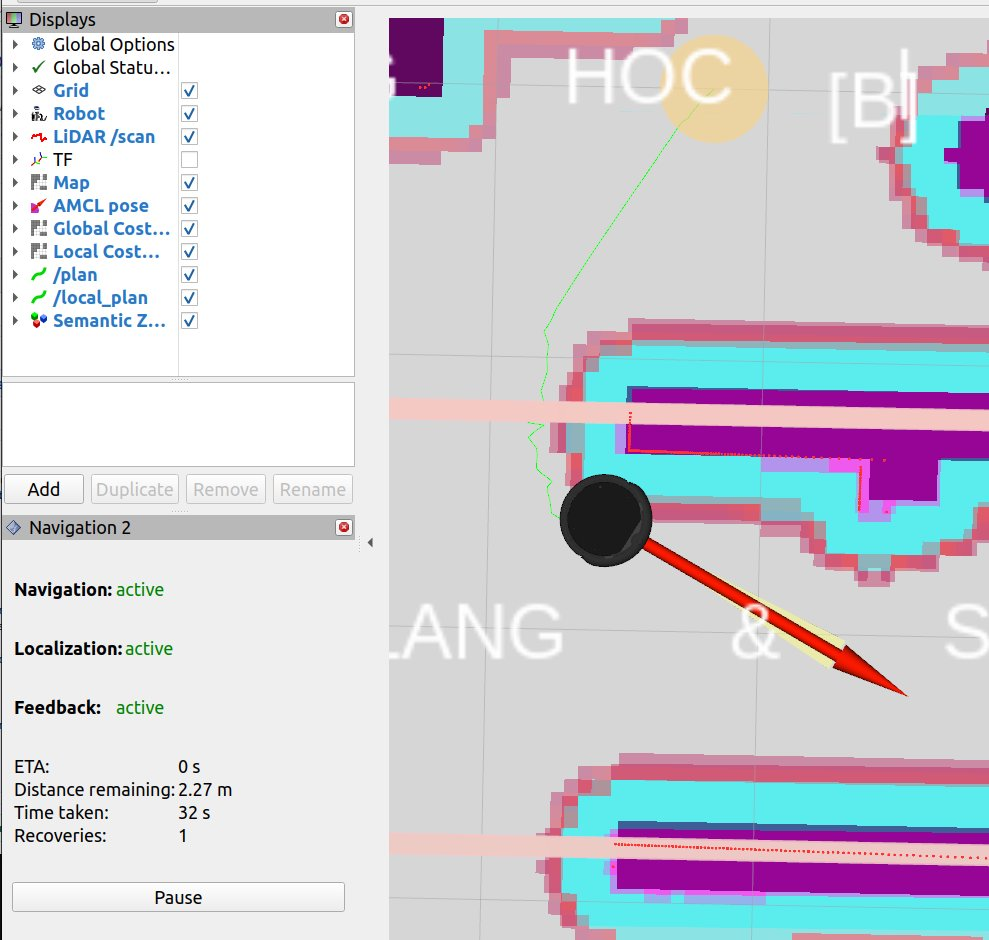
\includegraphics[width=\textwidth]{figures/run_rviz_amcl_costmap.jpg}
    \caption{Bám vết điều khiển Nav2 DWB Controller mượt mà lướt qua cửa phòng hẹp không kẹt góc.}
    \label{fig:rviz_dwb}
\end{subfigure}
\caption{Bộ ảnh thực nghiệm ghi nhận toàn bộ quá trình vận hành của TurtleBot 4 trong hệ thống điều hướng ngữ nghĩa.}
\label{fig:experiments}
\end{figure}
